\documentclass[a4paper, 12pt]{report}
\usepackage[T1]{fontenc} 
% \usepackage[icelandic]{babel}
\usepackage{latexsym,amssymb,amsmath,amsthm}
\usepackage{graphicx}
\usepackage{hyperref}
\usepackage{enumerate}
\usepackage{pgfplots}
\usepackage{nicefrac}
\usepackage{derivative}
\usepackage{setspace}
\usepackage{mathrsfs}
\usepackage{newtxtext, newtxmath}
\usepackage{tabularx}
\usepackage{authblk}

\usepackage{algorithm}
\usepackage{algpseudocodex}
\usepackage[hang,flushmargin]{footmisc}

\pgfplotsset{compat=1.17}
\setlength{\jot}{1em}

\title{\textsc{Simulating the Evolution of\\ Neural Pathways and Structures} \\ \vspace*{10mm} \Large Development Journal}
\author[1]{Kári Hlynsson}
\author[2]{Young Jun Lee}
\affil[1]{University of Iceland, Department of Mathematics}
\affil[2]{University of Oxford, Department of Biology}
\date{}

\newtheorem{theorem}{Theorem}
\newtheorem{corollary}{Corollary}
\newtheorem{proposition}{Proposition}

\theoremstyle{definition}
\newtheorem{definition}{Definition}
\newtheorem*{remark}{Remark}

\let\oldproofname=\proofname
\renewcommand{\proofname}{\rm\bf{\oldproofname}}


\begin{document}

\maketitle

\onehalfspacing
\newpage

\tableofcontents

\newpage
\chapter*{Index of notation}
\renewcommand{\arraystretch}{1.7}
\begin{table}[ht!]
    \centering
    \begin{tabularx}{\textwidth}{l X}
      \textsc{Abbreviation} & \textsc{Definition} \\
      $\mathscr E = [0;w] \times [0;h]$ & Environment with \emph{width} $w$ and \emph{height} $h$. The environment
                                           can also be expressed as the set of locations $\ell$ such that $\mathscr E = \{\ell := \langle x_i, y_j \rangle \mid x_i \in [0;w] \land y_j \in [0;h]\rangle\}$ \\
      $n$                                & Size of the population. \\
      $E = (e_x, e_y)$                  & An entity with $x$ and $y$ coordinates in the environment such that $\ell_{E} \in \mathscr E$ ($\ell_E$ is the location which corresponds to the entity's location) \\
      $\mathbf C = \{C_1, \ldots, C_k\}$ & The partition of $\mathscr E$ into $k$ chunks $C_1, \ldots, C_k$ such that $\bigcap_{i = 1}^k C_i = \emptyset$ and $\bigcup_{i = 1}^k C_i = \mathscr E$, i.e. the
                                            \emph{set of chunks} $\mathbf C$ forms a complete partition of $\mathscr E$. \\
      $\mathbf O = \{O_1, \ldots, O_n\}$ & The population, the set of all organisms present within the environment. \\
      $\theta_R = \frac{1}{\delta_R}$    & An organism's \emph{ray resolution}. The ray resolution is defined as the inverse of the angle between the uniformly spaced sensory rays, $\delta_R$ which construct 
                                           the organism's sensory field. The higher the value of $\theta_R$, the more rays in the sensory field and vice versa. \\
      $\mathcal P: \mathbf O \to \ell$   & Positional mapping. Returns vector representation of an entity's location at some point in time. Note that $\mathcal P$ is a random variable.
    \end{tabularx}
\end{table}

\newpage
\chapter*{Common Acronyms}
\begin{table}[ht!]
    \centering
    \begin{tabularx}{\textwidth}{l X}
      \textsc{Acronym} & \textsc{Definition} \\
      CBS & Chunk-Based System \\
      UGP & Undirected-Graph Partitioning \\
      BFS & Breadth-First Search
    \end{tabularx}
\end{table}


\newpage

\chapter{Theoretical Basis}
\section{Note}
Hello there Jun

\noindent
This is an \textsc{\huge EXTREMELY} primitive draft.

\noindent
None of this final and subject to changes as we cooperate on this project.

\noindent
I also want to apologize for the common abbreviatons section, its a load of cowdung
but I feel we will need this to make our lives easier later on.


\chapter{Model Outline}
\section{Model Outline}
The aim of the model is to study the natural evolution of neural pathways in a population of organism
when exposed to survivalistic conditions. A rigid logical and syntactical foundation will make all succeeding
articulation on the model parameters and attributes easier. We therefore dedicate this first section towards
establishing a foundation of terms and definitions which we build on later.
\par The most critical aspects of the model we define here is the \emph{environment} and the \emph{entities} contained
therein. Neglecting any elevation, we define the environment as the bounded subset of the Cartesian plane, which we symbolize
$\mathscr E$ \footnote{Although elevation certainly plays a vital role in the foraging patterns of organisms in natural environments, we refrain
from its implementation as it only adds a level of complexity to the model design while minimally increasing simulation findings.}.
\par Contained within the environment are \emph{entities} which we can think of as actors within the simulation. The two types that occur
in this model are \emph{organisms} and \emph{food}. Again, a simple intuitive definition is that the organism is an individual of a species
present within the environment and nutrition is the foodstuffs which it consumes to gain energy and thus survive.
\par Entities can be divided into two types: \emph{organisms} and \emph{food}. What follows is simple: organisms are motile, can sense their surroundings
and consume food to gain energy. On the other hand, food has none of these qualities. We represent an entity as the object $E$, while organisms are denoted
$O$ and food by $F$.

\section{Simulation Phases}
\subsection{Foraging phase}
\subsection{Reproductive phase}
For your contemplation (Jun, if you're reading this): I've thought of dividing the simulation into a \emph{foraging phase}, where organisms roam around and collect food.
If they don't get any or deplete their energy, they die. Once the foraging phase is over, the \emph{reproductive phase} starts, where remaining energy is a measure of how
likely organisms are to find a partner and reproduce (this is of course a simplication, there are many other ways to go about this I'm sure). This way, we don't have to make
the reproduction itself an extreme pain (organisms having to find each other, etc.) This would mean that the reproductive phase is not carried out in the "plane" where the simulation
occurs but rather "off screen" where its just a bunch of calculations really.
\par On the other hand it might make for some really interesting data if we were to assign individuals genders and they would map their current energy level and the gender of individuals
in their sensory field and allow for them to reproduce "in the field" lol. Let me know what you think!
\par Of course, if this fails to capture your attention (which I totally understand btw, I tend to glimpse through text without realizing what I'm reading, I'll definitely show this paragraph to you
the next time we talk, making for a really awkward $x$ seconds, depending on how fast you read.)

\section{Runtime optimization}
One of the run-ins we've had so far is determining how to design the sensory mapping capabilities of organisms within the environment. By sensory mapping, I am referring to the organism's ability to sense its
proximal surroundings, sensing the proximity and types of the various entities they may encounter. This will be fed into their neural network, which outputs some response which instructs the organism how to behave
given its current surroundings.
\par The first attempt I made was in the days where the environment was grid-based instead of a float-based environment. There, sensory mapping was quite easy as all that had to be done was inspect the proximal tiles
and check for the entity type present in the tile. This is not possible in the float-based environment, so we propose another solution.
\par An excellent idea you came up with was the idea of partitioning the environment into separate chunks, which organisms restrict their sensory mapping to unless there sensory fields intersect another adjacent chunk
(more on that later). We will start by discussing this idea, which as you will see, will be of great use.

\subsection{Chunk partitioning}
In this section, we will be doing a mathematical analysis of the chunk system to see how it will benefit the simulation. To start off, we inspect what fundamental laws apply to this system.

\begin{proposition}
    Let $\mathscr E$ be an environment paritioned into $k$ chunks such that $\mathbf C = \{C_1, \ldots, C_k\}$. The probability of an entity being present in a generic chunk $C_i$ equals $1/k$, i.e.
    \[
        \textnormal{Pr}\{E \in C_i\} = \frac 1k
    \]
\end{proposition}

\begin{proof}
    Let $\mathscr E$ be the space $[0; w] \times [0;h]$ with $\text{area}(\mathscr E) = wh$ and the partition $\mathbf C$. Under the assumption that the chunks
    are of uniform size, we assume
    \[
        \text{area}(C_i) = \frac{\text{area}(\mathscr E)}{k} \tag{\textasteriskcentered}
    \]
    for all $C_i \in \mathbf C$ where $i \in [1; k]$. Under conventional probability theory, we can express the probability of an entity being in a generic chunk as
    the area of that particular chunk over the area of the environment, i.e.
    \begin{align*}
        \text{Pr}\{E \in C_i\} &= \frac{|C_i|}{|\mathscr E|} \\
                               &= \frac{\text{area}(C_i)}{\text{area}(\mathscr E)} \\
                               &= \frac{1}{k}
    \end{align*}
    The result of the calculations above are immediate of the definition of the area of the chunks, which is derived in (\textasteriskcentered).
\end{proof}

\begin{definition}[Chunk load]
    The random variable $\mathcal L$, or the \emph{chunk load} of some generic chunk $C_i$,
    denotes the number of entities contained within the chunk. Immediate of proposition 1,
    we have that $\mathcal L \sim \text{Bin}(n, 1/k)$, where $n$ is the total number of entities
    in the environment. \footnote{Note that this assumes the uniform distribution of entities within
    the environment, which is obviously true. This is because there is no logical restraint on where an
    entity can be at any given time, i.e. there is not a consistent probabilistic hindrance in an entity having a certain position.}
\end{definition}

\begin{figure}[ht!]
    \centering
    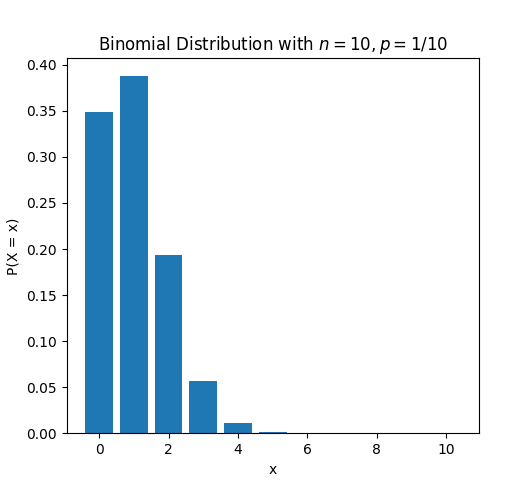
\includegraphics[width=0.6\textwidth]{img/binomialdistribution.png}
    \caption{An example binomial distribution}
\end{figure}

\subsection{Adjacent chunk loading}
The following algorithm can be easily 

\section{Performance comparison}

\appendix

\newpage

\chapter{Preliminaries}
\begin{definition}[Probability]
    Let $\omega$ be some event from the probability space $\Omega$. We represent
    the probability of the event $\omega$ occuring using the notation $\text{Pr}\{\omega\} = x$
    where $x \in [0;1]$.
\end{definition}

\begin{definition}[Random variable]
    A random variable $X$ is the mapping from the probability space $\Omega$ to the real number
    line, i.e. $X: \Omega \to \mathbb R$.
\end{definition}

\begin{remark}
    An example of a random variable is the varying height of a population, where $\Omega$ is the
    space of all possible outcomes and the random variable $H$ (height) is for example 180 cm, or 157 cm. 
\end{remark}

\begin{definition}[Expected value]
    Let $X$ be a random variable. The expected value is denoted $\mathbb E[X]$.
\end{definition}

\begin{definition}[Probability distribution]
    Let $X$ be a random variable. When it follows for example the Poisson distribution, we write
    $X \sim \text{Poisson}(\lambda)$.
\end{definition}

\end{document}